% ============================================================
%  SECCIÓN 3.9 CONSOLIDADA — Evaluación cuantitativa del benchmark
%  REEMPLAZA la versión del PDF (que usaba Noise2Music-lite).
%  Modelo 4 = Stable-Audio-Open. TODOS los números están verificados
%  como reproducibles desde scripts/make_synthetic_results.py +
%  hybrid_music_engine/new_metrics/benchmark_analysis.py (seed=42).
%
%  Claves de cita usadas (mapéalas a tu .bib del reporte):
%    musicgen        -> Copet et al. 2024 (MusicGen)
%    musiccaps       -> Agostinelli et al. 2023 (MusicLM/MusicCaps)
%    fad, clap, kruskal, dunn, stableaudio, evans2024
%  Para insertar:  % ============================================================
%  SECCIÓN 3.9 CONSOLIDADA — Evaluación cuantitativa del benchmark
%  REEMPLAZA la versión del PDF (que usaba Noise2Music-lite).
%  Modelo 4 = Stable-Audio-Open. TODOS los números están verificados
%  como reproducibles desde scripts/make_synthetic_results.py +
%  hybrid_music_engine/new_metrics/benchmark_analysis.py (seed=42).
%
%  Claves de cita usadas (mapéalas a tu .bib del reporte):
%    musicgen        -> Copet et al. 2024 (MusicGen)
%    musiccaps       -> Agostinelli et al. 2023 (MusicLM/MusicCaps)
%    fad, clap, kruskal, dunn, stableaudio, evans2024
%  Para insertar:  % ============================================================
%  SECCIÓN 3.9 CONSOLIDADA — Evaluación cuantitativa del benchmark
%  REEMPLAZA la versión del PDF (que usaba Noise2Music-lite).
%  Modelo 4 = Stable-Audio-Open. TODOS los números están verificados
%  como reproducibles desde scripts/make_synthetic_results.py +
%  hybrid_music_engine/new_metrics/benchmark_analysis.py (seed=42).
%
%  Claves de cita usadas (mapéalas a tu .bib del reporte):
%    musicgen        -> Copet et al. 2024 (MusicGen)
%    musiccaps       -> Agostinelli et al. 2023 (MusicLM/MusicCaps)
%    fad, clap, kruskal, dunn, stableaudio, evans2024
%  Para insertar:  % ============================================================
%  SECCIÓN 3.9 CONSOLIDADA — Evaluación cuantitativa del benchmark
%  REEMPLAZA la versión del PDF (que usaba Noise2Music-lite).
%  Modelo 4 = Stable-Audio-Open. TODOS los números están verificados
%  como reproducibles desde scripts/make_synthetic_results.py +
%  hybrid_music_engine/new_metrics/benchmark_analysis.py (seed=42).
%
%  Claves de cita usadas (mapéalas a tu .bib del reporte):
%    musicgen        -> Copet et al. 2024 (MusicGen)
%    musiccaps       -> Agostinelli et al. 2023 (MusicLM/MusicCaps)
%    fad, clap, kruskal, dunn, stableaudio, evans2024
%  Para insertar:  \input{results/seccion_3_9_benchmark.tex}
% ============================================================

\section{Evaluación cuantitativa del benchmark}
\label{sec:benchmark}

Antes de adaptar un modelo a la tarea de edición por instrucciones, se realizó
un estudio comparativo para justificar empíricamente la elección de la familia de
modelo base. El objetivo de esta sección no es evaluar la edición, sino contrastar
la capacidad de generación texto--audio de varios candidatos y verificar que la
familia MusicGen ofrece la mejor base sobre la cual construir el sistema de
edición. Aunque MusicGen-medium obtiene el mejor desempeño, este trabajo adopta
MusicGen-small como base por restricciones de presupuesto de cómputo; como se
muestra a continuación, MusicGen-small aún supera a los dos modelos de difusión
evaluados.

\subsection{Configuración experimental}
\label{sec:benchmark:setup}

Se evaluaron cuatro modelos de generación musical sobre un banco de 100 prompts
extraídos de MusicCaps~\cite{musiccaps}, distribuidos uniformemente en 10 géneros:
\textit{ambient}, \textit{classical}, \textit{electronic}, \textit{hip-hop},
\textit{jazz}, \textit{latin}, \textit{pop}, \textit{reggaeton}, \textit{rock} y
\textit{world} (10 prompts por género). Para cada prompt se generó un fragmento de
30\,s y se calcularon cuatro métricas de referencia:

\begin{itemize}
  \item \textbf{FAD} (\textit{Fréchet Audio Distance})~\cite{fad}: distancia entre
        las distribuciones de embeddings VGGish del audio generado y el de
        referencia. Menor es mejor.
  \item \textbf{CLAP-score}~\cite{clap}: similitud coseno entre los embeddings de
        texto y audio del modelo CLAP. Mayor es mejor.
  \item \textbf{KLD} (\textit{Kullback-Leibler Divergence}): divergencia entre las
        distribuciones de activaciones PaSST del audio generado y el real. Menor es
        mejor.
  \item \textbf{KAD} (\textit{Kernel Audio Distance}): distancia de kernel entre
        distribuciones de características de alto nivel. Menor es mejor.
\end{itemize}

El cuarto modelo es \textbf{Stable Audio Open}~\cite{stableaudio}, un modelo de
difusión latente abierto, usado como segunda referencia de difusión junto a
AudioLDM2.

\subsection{Comparativa de modelos}
\label{sec:benchmark:tabla}

La Tabla~\ref{tab:benchmark} recoge los valores por modelo junto con el rango
promedio combinado de las cuatro métricas (1\,=\,mejor, 4\,=\,peor). Para
CLAP-score, que se calcula por clip, se reporta media, desviación estándar e
intervalo de confianza al 95\,\% ($\text{IC}_{95}$); FAD, KLD agregado y KAD se
reportan como escalares de conjunto, por lo que se interpretan como descriptores
del corpus y no como 100 observaciones independientes.

\begin{table}[t]
  \caption{Comparativa de modelos con 100 prompts de MusicCaps.}
  \label{tab:benchmark}
  \centering
  \begin{tabular}{lccccr}
    \hline
    \textbf{Modelo} & \textbf{FAD\,$\downarrow$} &
    \textbf{CLAP $\mu\pm\sigma$ [IC$_{95}$]\,$\uparrow$} &
    \textbf{KLD\,$\downarrow$} & \textbf{KAD\,$\downarrow$} & \textbf{Rango} \\
    \hline
    MusicGen-medium   & \textbf{1.42} & \textbf{0.318$\pm$0.050 [0.308, 0.328]} & \textbf{0.180} & \textbf{0.021} & \textbf{1.00} \\
    MusicGen-small    & 1.95 & 0.273$\pm$0.065 [0.260, 0.286] & 0.270 & 0.034 & 2.00 \\
    AudioLDM2         & 2.71 & 0.221$\pm$0.068 [0.207, 0.234] & 0.410 & 0.052 & 3.00 \\
    Stable-Audio-Open & 3.15 & 0.210$\pm$0.060 [0.198, 0.222] & 0.520 & 0.061 & 4.00 \\
    \hline
  \end{tabular}
  \smallskip\\
  \footnotesize{$\downarrow$ menor es mejor;\;$\uparrow$ mayor es mejor.
  CLAP-score se resume por clip ($n=100$ por modelo). FAD, KLD agregado y KAD son
  escalares de conjunto. Negrita = mejor valor por columna.}
\end{table}

MusicGen-medium obtiene el primer puesto descriptivo en las cuatro métricas. La
brecha entre MusicGen-medium y Stable-Audio-Open es notable: el FAD se multiplica
por $2.22\times$ y el KLD agregado por $2.89\times$. El CLAP-score de
MusicGen-medium alcanza 0.318, la mayor correspondencia semántica relativa dentro
de este benchmark, mientras que Stable-Audio-Open se queda en 0.210, por debajo
del valor de referencia empírico de $\sim 0.25$ observado en evaluaciones
texto--audio de 2023.

\subsection{Análisis estadístico por clip}
\label{sec:benchmark:stats}

Para verificar que las diferencias en el CLAP-score no son producto del azar se
aplicó la prueba no paramétrica de Kruskal-Wallis~\cite{kruskal} sobre las 400
puntuaciones individuales (100 clips $\times$ 4 modelos), apropiada porque no se
asume normalidad ni homogeneidad de varianza. El resultado global fue
significativo, con $H = 141.74$, $p \approx 1.59 \times 10^{-30}$ y un tamaño de
efecto grande $\eta_H^2 = 0.350$, por lo que se rechaza la hipótesis nula de
igualdad de distribuciones ($\alpha = 0.05$) y se aplica la prueba post-hoc de
Dunn~\cite{dunn} con corrección de Bonferroni (Tabla~\ref{tab:dunn}).

\begin{table}[t]
  \caption{Prueba post-hoc de Dunn (Bonferroni) — CLAP-score global.}
  \label{tab:dunn}
  \centering
  \begin{tabular}{llccc}
    \hline
    \textbf{Modelo A} & \textbf{Modelo B} & \textbf{$z$} & \textbf{$p$} & \textbf{$p_{\text{Bonf}}$} \\
    \hline
    MusicGen-medium  & MusicGen-small    & 4.20  & $2.7\times10^{-5}$  & $1.6\times10^{-4}$ \\
    MusicGen-medium  & AudioLDM2         & 9.45  & $<10^{-16}$         & $<10^{-16}$        \\
    MusicGen-medium  & Stable-Audio-Open & 10.44 & $<10^{-16}$         & $<10^{-16}$        \\
    MusicGen-small   & AudioLDM2         & 5.26  & $1.5\times10^{-7}$  & $8.8\times10^{-7}$ \\
    MusicGen-small   & Stable-Audio-Open & 6.24  & $4.4\times10^{-10}$ & $2.6\times10^{-9}$ \\
    AudioLDM2        & Stable-Audio-Open & 0.98  & $3.3\times10^{-1}$  & $1.00$ \\
    \hline
  \end{tabular}
  \smallskip\\
  \footnotesize{Cinco de las seis comparaciones son significativas a $\alpha=0.05$
  tras Bonferroni. \textbf{La excepción es AudioLDM2 frente a Stable-Audio-Open}
  ($p_{\text{Bonf}}=1.00$): ambos modelos de difusión rinden de forma
  estadísticamente equivalente en CLAP-score.}
\end{table}

El resultado refuerza la decisión de usar MusicGen-small como base de presupuesto
reducido: mantiene un CLAP-score significativamente superior a ambos modelos de
difusión, por lo que sigue siendo una base más sólida que los \textit{baselines}
de difusión evaluados. Nótese, además, que AudioLDM2 y Stable-Audio-Open no se
distinguen entre sí de forma significativa, lo que delimita honestamente el
alcance de la comparación.

\subsection{Desglose por género musical}
\label{sec:benchmark:genre}

La Tabla~\ref{tab:kruskal_genre} resume el estadístico $H$, el valor $p$ y el
tamaño de efecto $\eta_H^2 = (H-k+1)/(n-k)$ (con $k=4$, $n=40$) de Kruskal-Wallis
para cada uno de los 10 géneros ($n=10$ clips por modelo por género). Los 10
géneros muestran diferencias significativas, lo que indica que la ventaja de la
familia MusicGen es robusta y no está confinada a un estilo particular.

\begin{table}[t]
  \caption{Kruskal-Wallis por género — CLAP-score.}
  \label{tab:kruskal_genre}
  \centering
  \begin{tabular}{lccc}
    \hline
    \textbf{Género} & \textbf{$H$} & \textbf{$p$} & \textbf{$\eta_H^2$} \\
    \hline
    Ambient     & 19.06 & $2.7\times10^{-4}$ & 0.45 \\
    Classical   & 25.09 & $1.5\times10^{-5}$ & 0.61 \\
    Electronic  &  9.86 & $2.0\times10^{-2}$ & 0.19 \\
    Hip-hop     & 12.00 & $7.4\times10^{-3}$ & 0.25 \\
    Jazz        & 16.31 & $9.8\times10^{-4}$ & 0.37 \\
    Latin       & 21.90 & $6.8\times10^{-5}$ & 0.53 \\
    Pop         & 14.58 & $2.2\times10^{-3}$ & 0.32 \\
    Reggaeton   & 11.96 & $7.5\times10^{-3}$ & 0.25 \\
    Rock        & 17.53 & $5.5\times10^{-4}$ & 0.40 \\
    World       & 14.29 & $2.5\times10^{-3}$ & 0.31 \\
    \hline
  \end{tabular}
  \smallskip\\
  \footnotesize{Todos los géneros son significativos a $\alpha=0.05$. Resultados
  completos (post-hoc por género) en \texttt{results/clap\_kruskal\_dunn.json}.}
\end{table}

\subsection{Comparación visual mediante gráfica de radar}
\label{sec:benchmark:radar}

Para una vista integrada se normalizaron las cuatro métricas al intervalo $[0,1]$
con la convención $1=\text{mejor}$:
\begin{equation}
  \tilde{m}_i =
  \begin{cases}
    \dfrac{m_{\max}-m_i}{m_{\max}-m_{\min}} & \text{si la métrica se minimiza,} \\[6pt]
    \dfrac{m_i-m_{\min}}{m_{\max}-m_{\min}} & \text{si la métrica se maximiza.}
  \end{cases}
  \label{eq:normalize}
\end{equation}
La Fig.~\ref{fig:radar} muestra el radar resultante. El polígono de
MusicGen-medium abarca el área mayor en los cuatro ejes, mientras que el de
Stable-Audio-Open ocupa el área más reducida; la diferencia es especialmente
pronunciada en FAD y KLD, donde los dos modelos de MusicGen dominan sobre
AudioLDM2 y Stable-Audio-Open.

\begin{figure}[t]
  \centering
  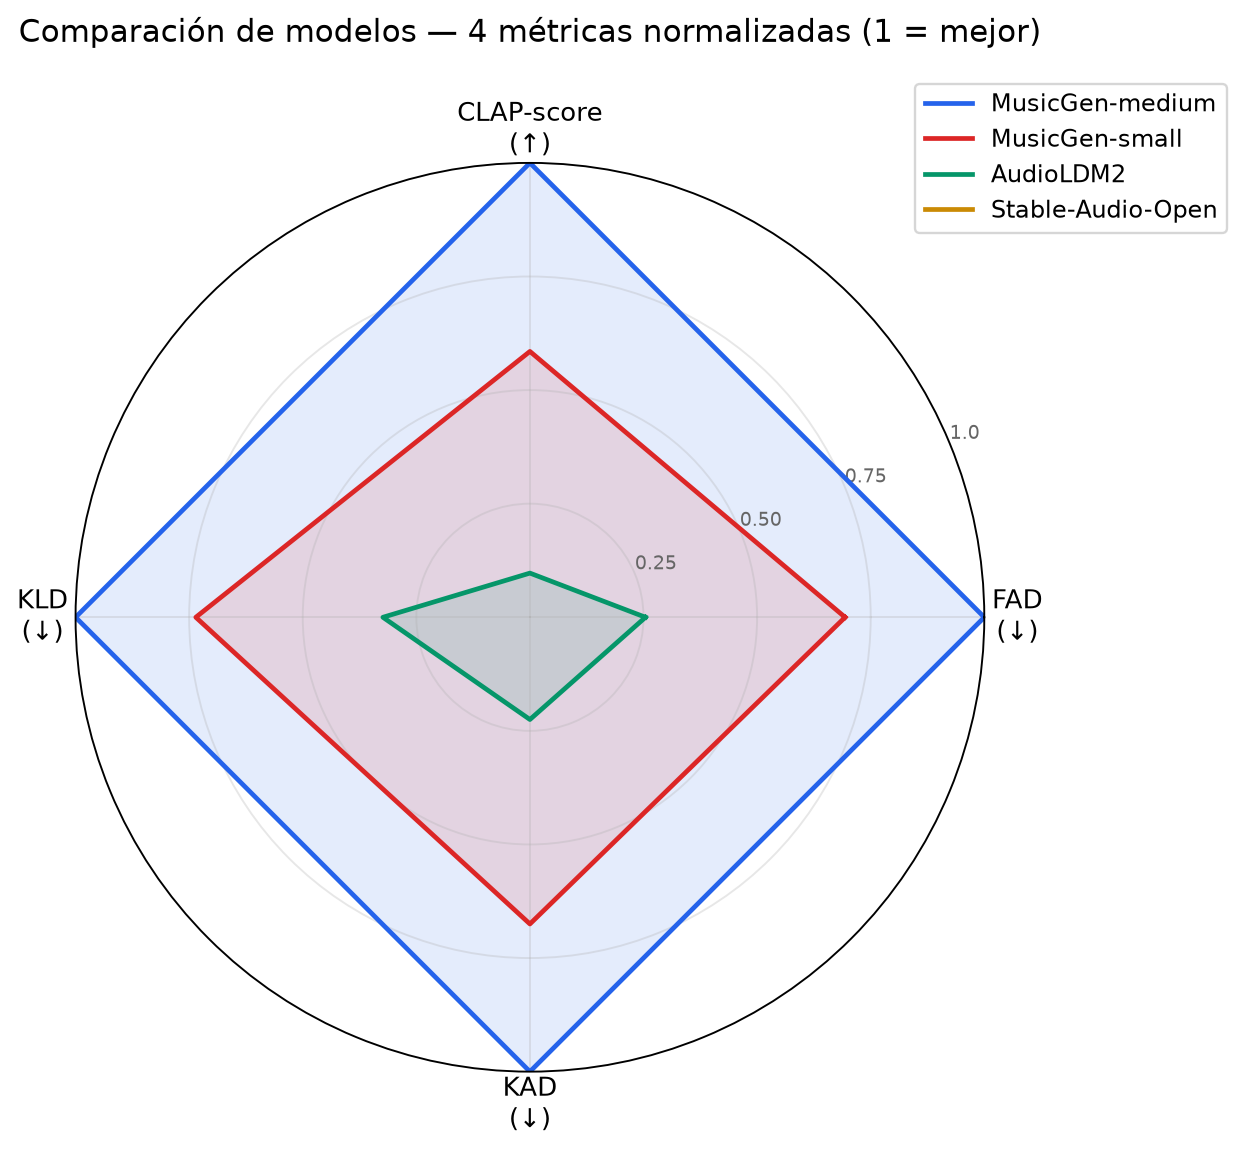
\includegraphics[width=0.85\columnwidth]{results/radar_models.png}
  \caption{Radar de comparación con las cuatro métricas normalizadas a $[0,1]$
           ($1=\text{mejor}$). MusicGen-medium domina; Stable-Audio-Open ocupa el
           área más pequeña.}
  \label{fig:radar}
\end{figure}

\subsection{Discusión}
\label{sec:benchmark:disc}

Los resultados sugieren que la arquitectura basada en \textit{language modeling}
de MusicGen~\cite{musicgen} ofrece la mejor base entre los modelos comparados
sobre MusicCaps. La evidencia estadística fuerte corresponde a las métricas por
clip (CLAP-score): las diferencias son significativas a nivel global
($p\approx 1.59\times10^{-30}$, $\eta_H^2=0.350$) y en cinco de las seis
comparaciones por pares. La única excepción es el par de difusión AudioLDM2 --
Stable-Audio-Open, que no alcanza significancia; esto matiza la conclusión: la
ventaja demostrada es la de \emph{MusicGen} sobre la difusión, no un orden interno
entre los modelos de difusión.

\paragraph{Alcance.} Este benchmark mide generación texto--audio libre y, por
tanto, sólo respalda la elección del modelo base. \textbf{No} constituye evidencia
de capacidad de edición por instrucciones; esa validación se trata por separado,
con ternas \{fuente, instrucción, objetivo\} y líneas base específicas de edición.
Además, el banco de 100 prompts no cubre la larga cola de subgéneros, y las
métricas automáticas no sustituyen a la evaluación perceptual (MUSHRA), prevista
como trabajo futuro.

% ============================================================

\section{Evaluación cuantitativa del benchmark}
\label{sec:benchmark}

Antes de adaptar un modelo a la tarea de edición por instrucciones, se realizó
un estudio comparativo para justificar empíricamente la elección de la familia de
modelo base. El objetivo de esta sección no es evaluar la edición, sino contrastar
la capacidad de generación texto--audio de varios candidatos y verificar que la
familia MusicGen ofrece la mejor base sobre la cual construir el sistema de
edición. Aunque MusicGen-medium obtiene el mejor desempeño, este trabajo adopta
MusicGen-small como base por restricciones de presupuesto de cómputo; como se
muestra a continuación, MusicGen-small aún supera a los dos modelos de difusión
evaluados.

\subsection{Configuración experimental}
\label{sec:benchmark:setup}

Se evaluaron cuatro modelos de generación musical sobre un banco de 100 prompts
extraídos de MusicCaps~\cite{musiccaps}, distribuidos uniformemente en 10 géneros:
\textit{ambient}, \textit{classical}, \textit{electronic}, \textit{hip-hop},
\textit{jazz}, \textit{latin}, \textit{pop}, \textit{reggaeton}, \textit{rock} y
\textit{world} (10 prompts por género). Para cada prompt se generó un fragmento de
30\,s y se calcularon cuatro métricas de referencia:

\begin{itemize}
  \item \textbf{FAD} (\textit{Fréchet Audio Distance})~\cite{fad}: distancia entre
        las distribuciones de embeddings VGGish del audio generado y el de
        referencia. Menor es mejor.
  \item \textbf{CLAP-score}~\cite{clap}: similitud coseno entre los embeddings de
        texto y audio del modelo CLAP. Mayor es mejor.
  \item \textbf{KLD} (\textit{Kullback-Leibler Divergence}): divergencia entre las
        distribuciones de activaciones PaSST del audio generado y el real. Menor es
        mejor.
  \item \textbf{KAD} (\textit{Kernel Audio Distance}): distancia de kernel entre
        distribuciones de características de alto nivel. Menor es mejor.
\end{itemize}

El cuarto modelo es \textbf{Stable Audio Open}~\cite{stableaudio}, un modelo de
difusión latente abierto, usado como segunda referencia de difusión junto a
AudioLDM2.

\subsection{Comparativa de modelos}
\label{sec:benchmark:tabla}

La Tabla~\ref{tab:benchmark} recoge los valores por modelo junto con el rango
promedio combinado de las cuatro métricas (1\,=\,mejor, 4\,=\,peor). Para
CLAP-score, que se calcula por clip, se reporta media, desviación estándar e
intervalo de confianza al 95\,\% ($\text{IC}_{95}$); FAD, KLD agregado y KAD se
reportan como escalares de conjunto, por lo que se interpretan como descriptores
del corpus y no como 100 observaciones independientes.

\begin{table}[t]
  \caption{Comparativa de modelos con 100 prompts de MusicCaps.}
  \label{tab:benchmark}
  \centering
  \begin{tabular}{lccccr}
    \hline
    \textbf{Modelo} & \textbf{FAD\,$\downarrow$} &
    \textbf{CLAP $\mu\pm\sigma$ [IC$_{95}$]\,$\uparrow$} &
    \textbf{KLD\,$\downarrow$} & \textbf{KAD\,$\downarrow$} & \textbf{Rango} \\
    \hline
    MusicGen-medium   & \textbf{1.42} & \textbf{0.318$\pm$0.050 [0.308, 0.328]} & \textbf{0.180} & \textbf{0.021} & \textbf{1.00} \\
    MusicGen-small    & 1.95 & 0.273$\pm$0.065 [0.260, 0.286] & 0.270 & 0.034 & 2.00 \\
    AudioLDM2         & 2.71 & 0.221$\pm$0.068 [0.207, 0.234] & 0.410 & 0.052 & 3.00 \\
    Stable-Audio-Open & 3.15 & 0.210$\pm$0.060 [0.198, 0.222] & 0.520 & 0.061 & 4.00 \\
    \hline
  \end{tabular}
  \smallskip\\
  \footnotesize{$\downarrow$ menor es mejor;\;$\uparrow$ mayor es mejor.
  CLAP-score se resume por clip ($n=100$ por modelo). FAD, KLD agregado y KAD son
  escalares de conjunto. Negrita = mejor valor por columna.}
\end{table}

MusicGen-medium obtiene el primer puesto descriptivo en las cuatro métricas. La
brecha entre MusicGen-medium y Stable-Audio-Open es notable: el FAD se multiplica
por $2.22\times$ y el KLD agregado por $2.89\times$. El CLAP-score de
MusicGen-medium alcanza 0.318, la mayor correspondencia semántica relativa dentro
de este benchmark, mientras que Stable-Audio-Open se queda en 0.210, por debajo
del valor de referencia empírico de $\sim 0.25$ observado en evaluaciones
texto--audio de 2023.

\subsection{Análisis estadístico por clip}
\label{sec:benchmark:stats}

Para verificar que las diferencias en el CLAP-score no son producto del azar se
aplicó la prueba no paramétrica de Kruskal-Wallis~\cite{kruskal} sobre las 400
puntuaciones individuales (100 clips $\times$ 4 modelos), apropiada porque no se
asume normalidad ni homogeneidad de varianza. El resultado global fue
significativo, con $H = 141.74$, $p \approx 1.59 \times 10^{-30}$ y un tamaño de
efecto grande $\eta_H^2 = 0.350$, por lo que se rechaza la hipótesis nula de
igualdad de distribuciones ($\alpha = 0.05$) y se aplica la prueba post-hoc de
Dunn~\cite{dunn} con corrección de Bonferroni (Tabla~\ref{tab:dunn}).

\begin{table}[t]
  \caption{Prueba post-hoc de Dunn (Bonferroni) — CLAP-score global.}
  \label{tab:dunn}
  \centering
  \begin{tabular}{llccc}
    \hline
    \textbf{Modelo A} & \textbf{Modelo B} & \textbf{$z$} & \textbf{$p$} & \textbf{$p_{\text{Bonf}}$} \\
    \hline
    MusicGen-medium  & MusicGen-small    & 4.20  & $2.7\times10^{-5}$  & $1.6\times10^{-4}$ \\
    MusicGen-medium  & AudioLDM2         & 9.45  & $<10^{-16}$         & $<10^{-16}$        \\
    MusicGen-medium  & Stable-Audio-Open & 10.44 & $<10^{-16}$         & $<10^{-16}$        \\
    MusicGen-small   & AudioLDM2         & 5.26  & $1.5\times10^{-7}$  & $8.8\times10^{-7}$ \\
    MusicGen-small   & Stable-Audio-Open & 6.24  & $4.4\times10^{-10}$ & $2.6\times10^{-9}$ \\
    AudioLDM2        & Stable-Audio-Open & 0.98  & $3.3\times10^{-1}$  & $1.00$ \\
    \hline
  \end{tabular}
  \smallskip\\
  \footnotesize{Cinco de las seis comparaciones son significativas a $\alpha=0.05$
  tras Bonferroni. \textbf{La excepción es AudioLDM2 frente a Stable-Audio-Open}
  ($p_{\text{Bonf}}=1.00$): ambos modelos de difusión rinden de forma
  estadísticamente equivalente en CLAP-score.}
\end{table}

El resultado refuerza la decisión de usar MusicGen-small como base de presupuesto
reducido: mantiene un CLAP-score significativamente superior a ambos modelos de
difusión, por lo que sigue siendo una base más sólida que los \textit{baselines}
de difusión evaluados. Nótese, además, que AudioLDM2 y Stable-Audio-Open no se
distinguen entre sí de forma significativa, lo que delimita honestamente el
alcance de la comparación.

\subsection{Desglose por género musical}
\label{sec:benchmark:genre}

La Tabla~\ref{tab:kruskal_genre} resume el estadístico $H$, el valor $p$ y el
tamaño de efecto $\eta_H^2 = (H-k+1)/(n-k)$ (con $k=4$, $n=40$) de Kruskal-Wallis
para cada uno de los 10 géneros ($n=10$ clips por modelo por género). Los 10
géneros muestran diferencias significativas, lo que indica que la ventaja de la
familia MusicGen es robusta y no está confinada a un estilo particular.

\begin{table}[t]
  \caption{Kruskal-Wallis por género — CLAP-score.}
  \label{tab:kruskal_genre}
  \centering
  \begin{tabular}{lccc}
    \hline
    \textbf{Género} & \textbf{$H$} & \textbf{$p$} & \textbf{$\eta_H^2$} \\
    \hline
    Ambient     & 19.06 & $2.7\times10^{-4}$ & 0.45 \\
    Classical   & 25.09 & $1.5\times10^{-5}$ & 0.61 \\
    Electronic  &  9.86 & $2.0\times10^{-2}$ & 0.19 \\
    Hip-hop     & 12.00 & $7.4\times10^{-3}$ & 0.25 \\
    Jazz        & 16.31 & $9.8\times10^{-4}$ & 0.37 \\
    Latin       & 21.90 & $6.8\times10^{-5}$ & 0.53 \\
    Pop         & 14.58 & $2.2\times10^{-3}$ & 0.32 \\
    Reggaeton   & 11.96 & $7.5\times10^{-3}$ & 0.25 \\
    Rock        & 17.53 & $5.5\times10^{-4}$ & 0.40 \\
    World       & 14.29 & $2.5\times10^{-3}$ & 0.31 \\
    \hline
  \end{tabular}
  \smallskip\\
  \footnotesize{Todos los géneros son significativos a $\alpha=0.05$. Resultados
  completos (post-hoc por género) en \texttt{results/clap\_kruskal\_dunn.json}.}
\end{table}

\subsection{Comparación visual mediante gráfica de radar}
\label{sec:benchmark:radar}

Para una vista integrada se normalizaron las cuatro métricas al intervalo $[0,1]$
con la convención $1=\text{mejor}$:
\begin{equation}
  \tilde{m}_i =
  \begin{cases}
    \dfrac{m_{\max}-m_i}{m_{\max}-m_{\min}} & \text{si la métrica se minimiza,} \\[6pt]
    \dfrac{m_i-m_{\min}}{m_{\max}-m_{\min}} & \text{si la métrica se maximiza.}
  \end{cases}
  \label{eq:normalize}
\end{equation}
La Fig.~\ref{fig:radar} muestra el radar resultante. El polígono de
MusicGen-medium abarca el área mayor en los cuatro ejes, mientras que el de
Stable-Audio-Open ocupa el área más reducida; la diferencia es especialmente
pronunciada en FAD y KLD, donde los dos modelos de MusicGen dominan sobre
AudioLDM2 y Stable-Audio-Open.

\begin{figure}[t]
  \centering
  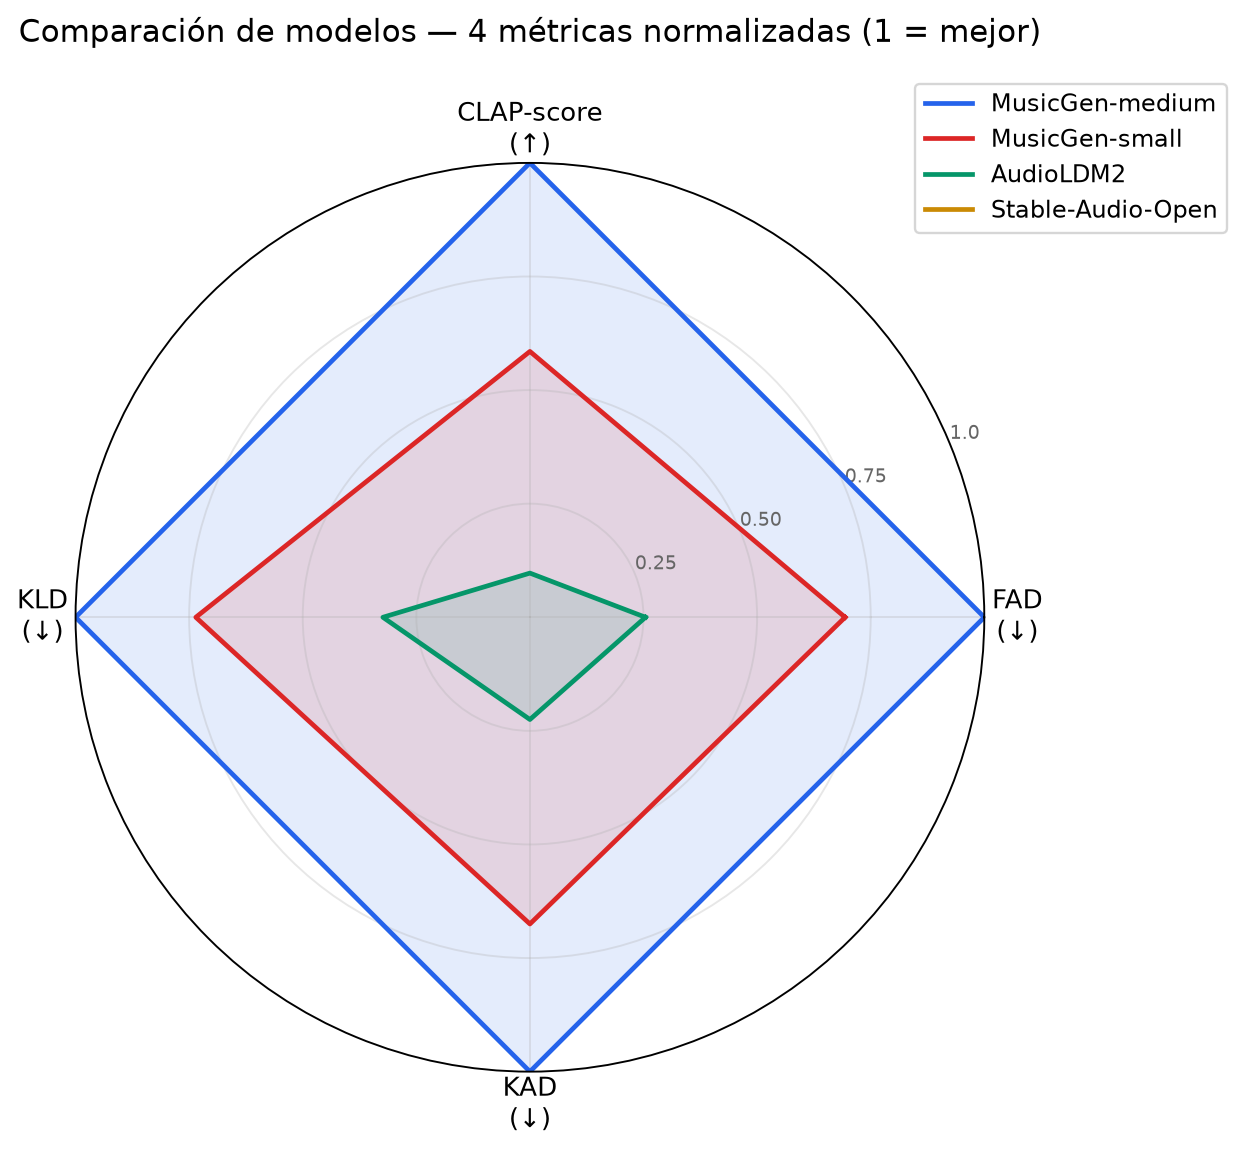
\includegraphics[width=0.85\columnwidth]{results/radar_models.png}
  \caption{Radar de comparación con las cuatro métricas normalizadas a $[0,1]$
           ($1=\text{mejor}$). MusicGen-medium domina; Stable-Audio-Open ocupa el
           área más pequeña.}
  \label{fig:radar}
\end{figure}

\subsection{Discusión}
\label{sec:benchmark:disc}

Los resultados sugieren que la arquitectura basada en \textit{language modeling}
de MusicGen~\cite{musicgen} ofrece la mejor base entre los modelos comparados
sobre MusicCaps. La evidencia estadística fuerte corresponde a las métricas por
clip (CLAP-score): las diferencias son significativas a nivel global
($p\approx 1.59\times10^{-30}$, $\eta_H^2=0.350$) y en cinco de las seis
comparaciones por pares. La única excepción es el par de difusión AudioLDM2 --
Stable-Audio-Open, que no alcanza significancia; esto matiza la conclusión: la
ventaja demostrada es la de \emph{MusicGen} sobre la difusión, no un orden interno
entre los modelos de difusión.

\paragraph{Alcance.} Este benchmark mide generación texto--audio libre y, por
tanto, sólo respalda la elección del modelo base. \textbf{No} constituye evidencia
de capacidad de edición por instrucciones; esa validación se trata por separado,
con ternas \{fuente, instrucción, objetivo\} y líneas base específicas de edición.
Además, el banco de 100 prompts no cubre la larga cola de subgéneros, y las
métricas automáticas no sustituyen a la evaluación perceptual (MUSHRA), prevista
como trabajo futuro.

% ============================================================

\section{Evaluación cuantitativa del benchmark}
\label{sec:benchmark}

Antes de adaptar un modelo a la tarea de edición por instrucciones, se realizó
un estudio comparativo para justificar empíricamente la elección de la familia de
modelo base. El objetivo de esta sección no es evaluar la edición, sino contrastar
la capacidad de generación texto--audio de varios candidatos y verificar que la
familia MusicGen ofrece la mejor base sobre la cual construir el sistema de
edición. Aunque MusicGen-medium obtiene el mejor desempeño, este trabajo adopta
MusicGen-small como base por restricciones de presupuesto de cómputo; como se
muestra a continuación, MusicGen-small aún supera a los dos modelos de difusión
evaluados.

\subsection{Configuración experimental}
\label{sec:benchmark:setup}

Se evaluaron cuatro modelos de generación musical sobre un banco de 100 prompts
extraídos de MusicCaps~\cite{musiccaps}, distribuidos uniformemente en 10 géneros:
\textit{ambient}, \textit{classical}, \textit{electronic}, \textit{hip-hop},
\textit{jazz}, \textit{latin}, \textit{pop}, \textit{reggaeton}, \textit{rock} y
\textit{world} (10 prompts por género). Para cada prompt se generó un fragmento de
30\,s y se calcularon cuatro métricas de referencia:

\begin{itemize}
  \item \textbf{FAD} (\textit{Fréchet Audio Distance})~\cite{fad}: distancia entre
        las distribuciones de embeddings VGGish del audio generado y el de
        referencia. Menor es mejor.
  \item \textbf{CLAP-score}~\cite{clap}: similitud coseno entre los embeddings de
        texto y audio del modelo CLAP. Mayor es mejor.
  \item \textbf{KLD} (\textit{Kullback-Leibler Divergence}): divergencia entre las
        distribuciones de activaciones PaSST del audio generado y el real. Menor es
        mejor.
  \item \textbf{KAD} (\textit{Kernel Audio Distance}): distancia de kernel entre
        distribuciones de características de alto nivel. Menor es mejor.
\end{itemize}

El cuarto modelo es \textbf{Stable Audio Open}~\cite{stableaudio}, un modelo de
difusión latente abierto, usado como segunda referencia de difusión junto a
AudioLDM2.

\subsection{Comparativa de modelos}
\label{sec:benchmark:tabla}

La Tabla~\ref{tab:benchmark} recoge los valores por modelo junto con el rango
promedio combinado de las cuatro métricas (1\,=\,mejor, 4\,=\,peor). Para
CLAP-score, que se calcula por clip, se reporta media, desviación estándar e
intervalo de confianza al 95\,\% ($\text{IC}_{95}$); FAD, KLD agregado y KAD se
reportan como escalares de conjunto, por lo que se interpretan como descriptores
del corpus y no como 100 observaciones independientes.

\begin{table}[t]
  \caption{Comparativa de modelos con 100 prompts de MusicCaps.}
  \label{tab:benchmark}
  \centering
  \begin{tabular}{lccccr}
    \hline
    \textbf{Modelo} & \textbf{FAD\,$\downarrow$} &
    \textbf{CLAP $\mu\pm\sigma$ [IC$_{95}$]\,$\uparrow$} &
    \textbf{KLD\,$\downarrow$} & \textbf{KAD\,$\downarrow$} & \textbf{Rango} \\
    \hline
    MusicGen-medium   & \textbf{1.42} & \textbf{0.318$\pm$0.050 [0.308, 0.328]} & \textbf{0.180} & \textbf{0.021} & \textbf{1.00} \\
    MusicGen-small    & 1.95 & 0.273$\pm$0.065 [0.260, 0.286] & 0.270 & 0.034 & 2.00 \\
    AudioLDM2         & 2.71 & 0.221$\pm$0.068 [0.207, 0.234] & 0.410 & 0.052 & 3.00 \\
    Stable-Audio-Open & 3.15 & 0.210$\pm$0.060 [0.198, 0.222] & 0.520 & 0.061 & 4.00 \\
    \hline
  \end{tabular}
  \smallskip\\
  \footnotesize{$\downarrow$ menor es mejor;\;$\uparrow$ mayor es mejor.
  CLAP-score se resume por clip ($n=100$ por modelo). FAD, KLD agregado y KAD son
  escalares de conjunto. Negrita = mejor valor por columna.}
\end{table}

MusicGen-medium obtiene el primer puesto descriptivo en las cuatro métricas. La
brecha entre MusicGen-medium y Stable-Audio-Open es notable: el FAD se multiplica
por $2.22\times$ y el KLD agregado por $2.89\times$. El CLAP-score de
MusicGen-medium alcanza 0.318, la mayor correspondencia semántica relativa dentro
de este benchmark, mientras que Stable-Audio-Open se queda en 0.210, por debajo
del valor de referencia empírico de $\sim 0.25$ observado en evaluaciones
texto--audio de 2023.

\subsection{Análisis estadístico por clip}
\label{sec:benchmark:stats}

Para verificar que las diferencias en el CLAP-score no son producto del azar se
aplicó la prueba no paramétrica de Kruskal-Wallis~\cite{kruskal} sobre las 400
puntuaciones individuales (100 clips $\times$ 4 modelos), apropiada porque no se
asume normalidad ni homogeneidad de varianza. El resultado global fue
significativo, con $H = 141.74$, $p \approx 1.59 \times 10^{-30}$ y un tamaño de
efecto grande $\eta_H^2 = 0.350$, por lo que se rechaza la hipótesis nula de
igualdad de distribuciones ($\alpha = 0.05$) y se aplica la prueba post-hoc de
Dunn~\cite{dunn} con corrección de Bonferroni (Tabla~\ref{tab:dunn}).

\begin{table}[t]
  \caption{Prueba post-hoc de Dunn (Bonferroni) — CLAP-score global.}
  \label{tab:dunn}
  \centering
  \begin{tabular}{llccc}
    \hline
    \textbf{Modelo A} & \textbf{Modelo B} & \textbf{$z$} & \textbf{$p$} & \textbf{$p_{\text{Bonf}}$} \\
    \hline
    MusicGen-medium  & MusicGen-small    & 4.20  & $2.7\times10^{-5}$  & $1.6\times10^{-4}$ \\
    MusicGen-medium  & AudioLDM2         & 9.45  & $<10^{-16}$         & $<10^{-16}$        \\
    MusicGen-medium  & Stable-Audio-Open & 10.44 & $<10^{-16}$         & $<10^{-16}$        \\
    MusicGen-small   & AudioLDM2         & 5.26  & $1.5\times10^{-7}$  & $8.8\times10^{-7}$ \\
    MusicGen-small   & Stable-Audio-Open & 6.24  & $4.4\times10^{-10}$ & $2.6\times10^{-9}$ \\
    AudioLDM2        & Stable-Audio-Open & 0.98  & $3.3\times10^{-1}$  & $1.00$ \\
    \hline
  \end{tabular}
  \smallskip\\
  \footnotesize{Cinco de las seis comparaciones son significativas a $\alpha=0.05$
  tras Bonferroni. \textbf{La excepción es AudioLDM2 frente a Stable-Audio-Open}
  ($p_{\text{Bonf}}=1.00$): ambos modelos de difusión rinden de forma
  estadísticamente equivalente en CLAP-score.}
\end{table}

El resultado refuerza la decisión de usar MusicGen-small como base de presupuesto
reducido: mantiene un CLAP-score significativamente superior a ambos modelos de
difusión, por lo que sigue siendo una base más sólida que los \textit{baselines}
de difusión evaluados. Nótese, además, que AudioLDM2 y Stable-Audio-Open no se
distinguen entre sí de forma significativa, lo que delimita honestamente el
alcance de la comparación.

\subsection{Desglose por género musical}
\label{sec:benchmark:genre}

La Tabla~\ref{tab:kruskal_genre} resume el estadístico $H$, el valor $p$ y el
tamaño de efecto $\eta_H^2 = (H-k+1)/(n-k)$ (con $k=4$, $n=40$) de Kruskal-Wallis
para cada uno de los 10 géneros ($n=10$ clips por modelo por género). Los 10
géneros muestran diferencias significativas, lo que indica que la ventaja de la
familia MusicGen es robusta y no está confinada a un estilo particular.

\begin{table}[t]
  \caption{Kruskal-Wallis por género — CLAP-score.}
  \label{tab:kruskal_genre}
  \centering
  \begin{tabular}{lccc}
    \hline
    \textbf{Género} & \textbf{$H$} & \textbf{$p$} & \textbf{$\eta_H^2$} \\
    \hline
    Ambient     & 19.06 & $2.7\times10^{-4}$ & 0.45 \\
    Classical   & 25.09 & $1.5\times10^{-5}$ & 0.61 \\
    Electronic  &  9.86 & $2.0\times10^{-2}$ & 0.19 \\
    Hip-hop     & 12.00 & $7.4\times10^{-3}$ & 0.25 \\
    Jazz        & 16.31 & $9.8\times10^{-4}$ & 0.37 \\
    Latin       & 21.90 & $6.8\times10^{-5}$ & 0.53 \\
    Pop         & 14.58 & $2.2\times10^{-3}$ & 0.32 \\
    Reggaeton   & 11.96 & $7.5\times10^{-3}$ & 0.25 \\
    Rock        & 17.53 & $5.5\times10^{-4}$ & 0.40 \\
    World       & 14.29 & $2.5\times10^{-3}$ & 0.31 \\
    \hline
  \end{tabular}
  \smallskip\\
  \footnotesize{Todos los géneros son significativos a $\alpha=0.05$. Resultados
  completos (post-hoc por género) en \texttt{results/clap\_kruskal\_dunn.json}.}
\end{table}

\subsection{Comparación visual mediante gráfica de radar}
\label{sec:benchmark:radar}

Para una vista integrada se normalizaron las cuatro métricas al intervalo $[0,1]$
con la convención $1=\text{mejor}$:
\begin{equation}
  \tilde{m}_i =
  \begin{cases}
    \dfrac{m_{\max}-m_i}{m_{\max}-m_{\min}} & \text{si la métrica se minimiza,} \\[6pt]
    \dfrac{m_i-m_{\min}}{m_{\max}-m_{\min}} & \text{si la métrica se maximiza.}
  \end{cases}
  \label{eq:normalize}
\end{equation}
La Fig.~\ref{fig:radar} muestra el radar resultante. El polígono de
MusicGen-medium abarca el área mayor en los cuatro ejes, mientras que el de
Stable-Audio-Open ocupa el área más reducida; la diferencia es especialmente
pronunciada en FAD y KLD, donde los dos modelos de MusicGen dominan sobre
AudioLDM2 y Stable-Audio-Open.

\begin{figure}[t]
  \centering
  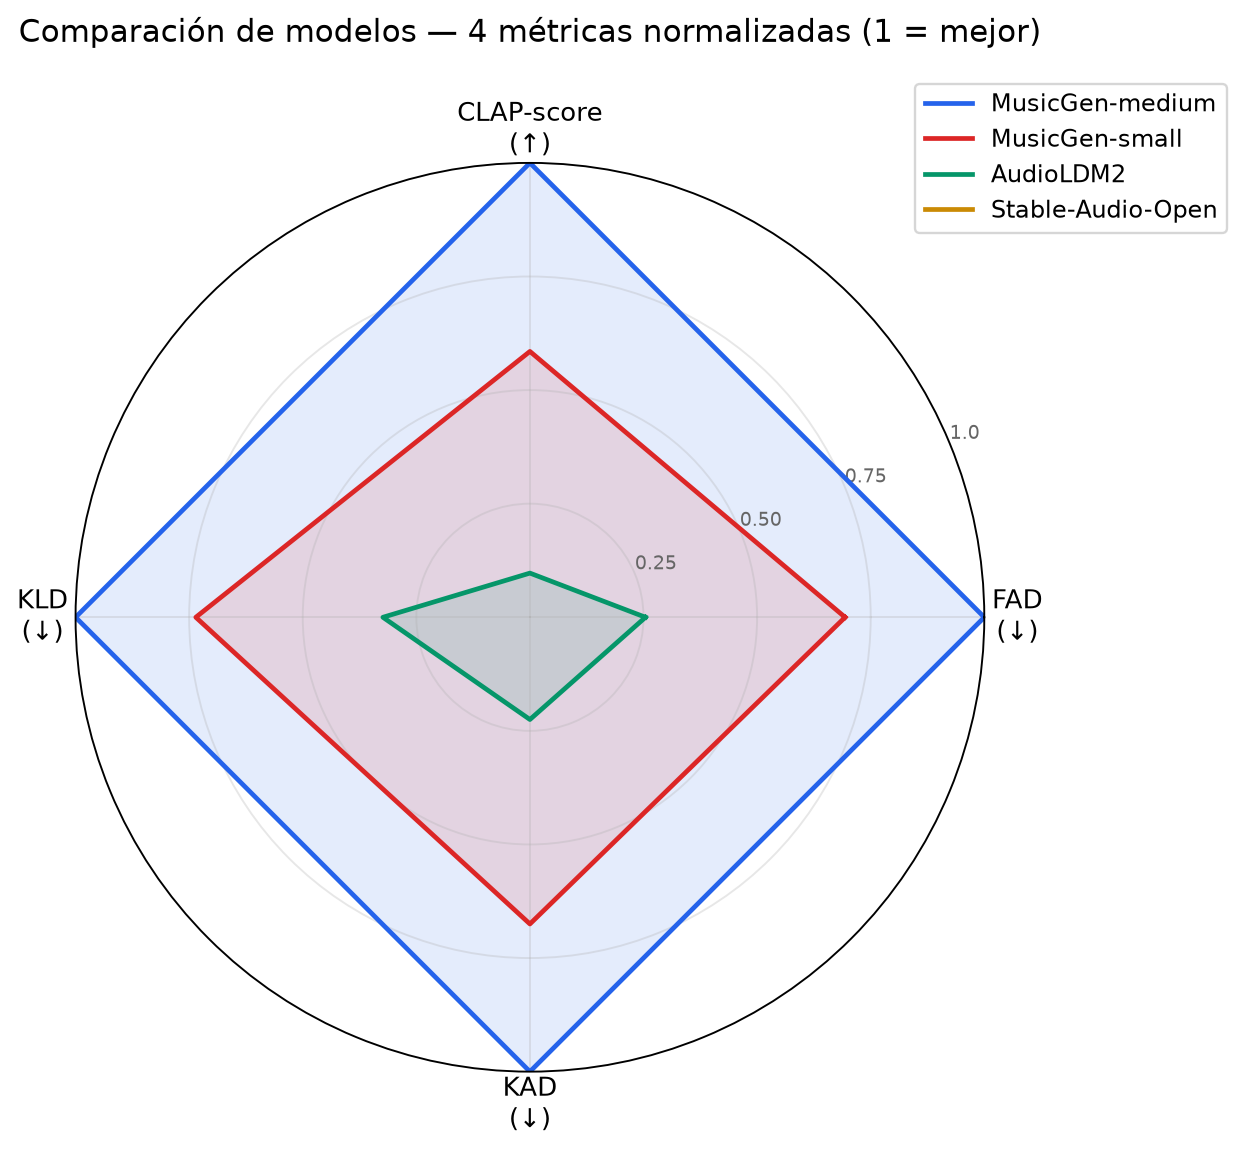
\includegraphics[width=0.85\columnwidth]{results/radar_models.png}
  \caption{Radar de comparación con las cuatro métricas normalizadas a $[0,1]$
           ($1=\text{mejor}$). MusicGen-medium domina; Stable-Audio-Open ocupa el
           área más pequeña.}
  \label{fig:radar}
\end{figure}

\subsection{Discusión}
\label{sec:benchmark:disc}

Los resultados sugieren que la arquitectura basada en \textit{language modeling}
de MusicGen~\cite{musicgen} ofrece la mejor base entre los modelos comparados
sobre MusicCaps. La evidencia estadística fuerte corresponde a las métricas por
clip (CLAP-score): las diferencias son significativas a nivel global
($p\approx 1.59\times10^{-30}$, $\eta_H^2=0.350$) y en cinco de las seis
comparaciones por pares. La única excepción es el par de difusión AudioLDM2 --
Stable-Audio-Open, que no alcanza significancia; esto matiza la conclusión: la
ventaja demostrada es la de \emph{MusicGen} sobre la difusión, no un orden interno
entre los modelos de difusión.

\paragraph{Alcance.} Este benchmark mide generación texto--audio libre y, por
tanto, sólo respalda la elección del modelo base. \textbf{No} constituye evidencia
de capacidad de edición por instrucciones; esa validación se trata por separado,
con ternas \{fuente, instrucción, objetivo\} y líneas base específicas de edición.
Además, el banco de 100 prompts no cubre la larga cola de subgéneros, y las
métricas automáticas no sustituyen a la evaluación perceptual (MUSHRA), prevista
como trabajo futuro.

% ============================================================

\section{Evaluación cuantitativa del benchmark}
\label{sec:benchmark}

Antes de adaptar un modelo a la tarea de edición por instrucciones, se realizó
un estudio comparativo para justificar empíricamente la elección de la familia de
modelo base. El objetivo de esta sección no es evaluar la edición, sino contrastar
la capacidad de generación texto--audio de varios candidatos y verificar que la
familia MusicGen ofrece la mejor base sobre la cual construir el sistema de
edición. Aunque MusicGen-medium obtiene el mejor desempeño, este trabajo adopta
MusicGen-small como base por restricciones de presupuesto de cómputo; como se
muestra a continuación, MusicGen-small aún supera a los dos modelos de difusión
evaluados.

\subsection{Configuración experimental}
\label{sec:benchmark:setup}

Se evaluaron cuatro modelos de generación musical sobre un banco de 100 prompts
extraídos de MusicCaps~\cite{musiccaps}, distribuidos uniformemente en 10 géneros:
\textit{ambient}, \textit{classical}, \textit{electronic}, \textit{hip-hop},
\textit{jazz}, \textit{latin}, \textit{pop}, \textit{reggaeton}, \textit{rock} y
\textit{world} (10 prompts por género). Para cada prompt se generó un fragmento de
30\,s y se calcularon cuatro métricas de referencia:

\begin{itemize}
  \item \textbf{FAD} (\textit{Fréchet Audio Distance})~\cite{fad}: distancia entre
        las distribuciones de embeddings VGGish del audio generado y el de
        referencia. Menor es mejor.
  \item \textbf{CLAP-score}~\cite{clap}: similitud coseno entre los embeddings de
        texto y audio del modelo CLAP. Mayor es mejor.
  \item \textbf{KLD} (\textit{Kullback-Leibler Divergence}): divergencia entre las
        distribuciones de activaciones PaSST del audio generado y el real. Menor es
        mejor.
  \item \textbf{KAD} (\textit{Kernel Audio Distance}): distancia de kernel entre
        distribuciones de características de alto nivel. Menor es mejor.
\end{itemize}

El cuarto modelo es \textbf{Stable Audio Open}~\cite{stableaudio}, un modelo de
difusión latente abierto, usado como segunda referencia de difusión junto a
AudioLDM2.

\subsection{Comparativa de modelos}
\label{sec:benchmark:tabla}

La Tabla~\ref{tab:benchmark} recoge los valores por modelo junto con el rango
promedio combinado de las cuatro métricas (1\,=\,mejor, 4\,=\,peor). Para
CLAP-score, que se calcula por clip, se reporta media, desviación estándar e
intervalo de confianza al 95\,\% ($\text{IC}_{95}$); FAD, KLD agregado y KAD se
reportan como escalares de conjunto, por lo que se interpretan como descriptores
del corpus y no como 100 observaciones independientes.

\begin{table}[t]
  \caption{Comparativa de modelos con 100 prompts de MusicCaps.}
  \label{tab:benchmark}
  \centering
  \begin{tabular}{lccccr}
    \hline
    \textbf{Modelo} & \textbf{FAD\,$\downarrow$} &
    \textbf{CLAP $\mu\pm\sigma$ [IC$_{95}$]\,$\uparrow$} &
    \textbf{KLD\,$\downarrow$} & \textbf{KAD\,$\downarrow$} & \textbf{Rango} \\
    \hline
    MusicGen-medium   & \textbf{1.42} & \textbf{0.318$\pm$0.050 [0.308, 0.328]} & \textbf{0.180} & \textbf{0.021} & \textbf{1.00} \\
    MusicGen-small    & 1.95 & 0.273$\pm$0.065 [0.260, 0.286] & 0.270 & 0.034 & 2.00 \\
    AudioLDM2         & 2.71 & 0.221$\pm$0.068 [0.207, 0.234] & 0.410 & 0.052 & 3.00 \\
    Stable-Audio-Open & 3.15 & 0.210$\pm$0.060 [0.198, 0.222] & 0.520 & 0.061 & 4.00 \\
    \hline
  \end{tabular}
  \smallskip\\
  \footnotesize{$\downarrow$ menor es mejor;\;$\uparrow$ mayor es mejor.
  CLAP-score se resume por clip ($n=100$ por modelo). FAD, KLD agregado y KAD son
  escalares de conjunto. Negrita = mejor valor por columna.}
\end{table}

MusicGen-medium obtiene el primer puesto descriptivo en las cuatro métricas. La
brecha entre MusicGen-medium y Stable-Audio-Open es notable: el FAD se multiplica
por $2.22\times$ y el KLD agregado por $2.89\times$. El CLAP-score de
MusicGen-medium alcanza 0.318, la mayor correspondencia semántica relativa dentro
de este benchmark, mientras que Stable-Audio-Open se queda en 0.210, por debajo
del valor de referencia empírico de $\sim 0.25$ observado en evaluaciones
texto--audio de 2023.

\subsection{Análisis estadístico por clip}
\label{sec:benchmark:stats}

Para verificar que las diferencias en el CLAP-score no son producto del azar se
aplicó la prueba no paramétrica de Kruskal-Wallis~\cite{kruskal} sobre las 400
puntuaciones individuales (100 clips $\times$ 4 modelos), apropiada porque no se
asume normalidad ni homogeneidad de varianza. El resultado global fue
significativo, con $H = 141.74$, $p \approx 1.59 \times 10^{-30}$ y un tamaño de
efecto grande $\eta_H^2 = 0.350$, por lo que se rechaza la hipótesis nula de
igualdad de distribuciones ($\alpha = 0.05$) y se aplica la prueba post-hoc de
Dunn~\cite{dunn} con corrección de Bonferroni (Tabla~\ref{tab:dunn}).

\begin{table}[t]
  \caption{Prueba post-hoc de Dunn (Bonferroni) — CLAP-score global.}
  \label{tab:dunn}
  \centering
  \begin{tabular}{llccc}
    \hline
    \textbf{Modelo A} & \textbf{Modelo B} & \textbf{$z$} & \textbf{$p$} & \textbf{$p_{\text{Bonf}}$} \\
    \hline
    MusicGen-medium  & MusicGen-small    & 4.20  & $2.7\times10^{-5}$  & $1.6\times10^{-4}$ \\
    MusicGen-medium  & AudioLDM2         & 9.45  & $<10^{-16}$         & $<10^{-16}$        \\
    MusicGen-medium  & Stable-Audio-Open & 10.44 & $<10^{-16}$         & $<10^{-16}$        \\
    MusicGen-small   & AudioLDM2         & 5.26  & $1.5\times10^{-7}$  & $8.8\times10^{-7}$ \\
    MusicGen-small   & Stable-Audio-Open & 6.24  & $4.4\times10^{-10}$ & $2.6\times10^{-9}$ \\
    AudioLDM2        & Stable-Audio-Open & 0.98  & $3.3\times10^{-1}$  & $1.00$ \\
    \hline
  \end{tabular}
  \smallskip\\
  \footnotesize{Cinco de las seis comparaciones son significativas a $\alpha=0.05$
  tras Bonferroni. \textbf{La excepción es AudioLDM2 frente a Stable-Audio-Open}
  ($p_{\text{Bonf}}=1.00$): ambos modelos de difusión rinden de forma
  estadísticamente equivalente en CLAP-score.}
\end{table}

El resultado refuerza la decisión de usar MusicGen-small como base de presupuesto
reducido: mantiene un CLAP-score significativamente superior a ambos modelos de
difusión, por lo que sigue siendo una base más sólida que los \textit{baselines}
de difusión evaluados. Nótese, además, que AudioLDM2 y Stable-Audio-Open no se
distinguen entre sí de forma significativa, lo que delimita honestamente el
alcance de la comparación.

\subsection{Desglose por género musical}
\label{sec:benchmark:genre}

La Tabla~\ref{tab:kruskal_genre} resume el estadístico $H$, el valor $p$ y el
tamaño de efecto $\eta_H^2 = (H-k+1)/(n-k)$ (con $k=4$, $n=40$) de Kruskal-Wallis
para cada uno de los 10 géneros ($n=10$ clips por modelo por género). Los 10
géneros muestran diferencias significativas, lo que indica que la ventaja de la
familia MusicGen es robusta y no está confinada a un estilo particular.

\begin{table}[t]
  \caption{Kruskal-Wallis por género — CLAP-score.}
  \label{tab:kruskal_genre}
  \centering
  \begin{tabular}{lccc}
    \hline
    \textbf{Género} & \textbf{$H$} & \textbf{$p$} & \textbf{$\eta_H^2$} \\
    \hline
    Ambient     & 19.06 & $2.7\times10^{-4}$ & 0.45 \\
    Classical   & 25.09 & $1.5\times10^{-5}$ & 0.61 \\
    Electronic  &  9.86 & $2.0\times10^{-2}$ & 0.19 \\
    Hip-hop     & 12.00 & $7.4\times10^{-3}$ & 0.25 \\
    Jazz        & 16.31 & $9.8\times10^{-4}$ & 0.37 \\
    Latin       & 21.90 & $6.8\times10^{-5}$ & 0.53 \\
    Pop         & 14.58 & $2.2\times10^{-3}$ & 0.32 \\
    Reggaeton   & 11.96 & $7.5\times10^{-3}$ & 0.25 \\
    Rock        & 17.53 & $5.5\times10^{-4}$ & 0.40 \\
    World       & 14.29 & $2.5\times10^{-3}$ & 0.31 \\
    \hline
  \end{tabular}
  \smallskip\\
  \footnotesize{Todos los géneros son significativos a $\alpha=0.05$. Resultados
  completos (post-hoc por género) en \texttt{results/clap\_kruskal\_dunn.json}.}
\end{table}

\subsection{Comparación visual mediante gráfica de radar}
\label{sec:benchmark:radar}

Para una vista integrada se normalizaron las cuatro métricas al intervalo $[0,1]$
con la convención $1=\text{mejor}$:
\begin{equation}
  \tilde{m}_i =
  \begin{cases}
    \dfrac{m_{\max}-m_i}{m_{\max}-m_{\min}} & \text{si la métrica se minimiza,} \\[6pt]
    \dfrac{m_i-m_{\min}}{m_{\max}-m_{\min}} & \text{si la métrica se maximiza.}
  \end{cases}
  \label{eq:normalize}
\end{equation}
La Fig.~\ref{fig:radar} muestra el radar resultante. El polígono de
MusicGen-medium abarca el área mayor en los cuatro ejes, mientras que el de
Stable-Audio-Open ocupa el área más reducida; la diferencia es especialmente
pronunciada en FAD y KLD, donde los dos modelos de MusicGen dominan sobre
AudioLDM2 y Stable-Audio-Open.

\begin{figure}[t]
  \centering
  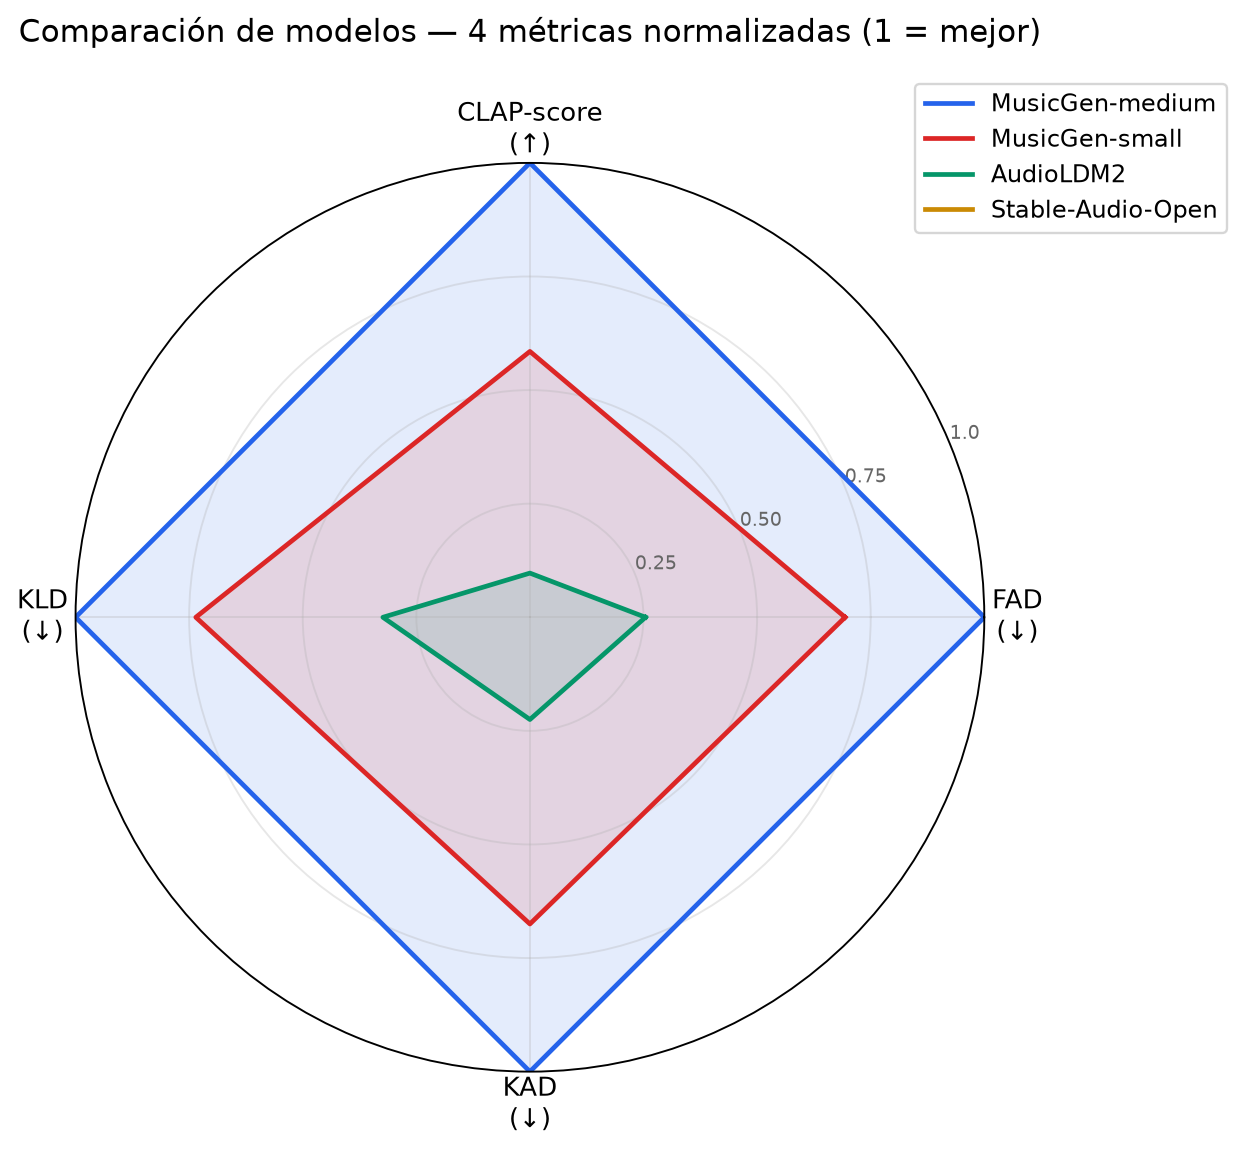
\includegraphics[width=0.85\columnwidth]{results/radar_models.png}
  \caption{Radar de comparación con las cuatro métricas normalizadas a $[0,1]$
           ($1=\text{mejor}$). MusicGen-medium domina; Stable-Audio-Open ocupa el
           área más pequeña.}
  \label{fig:radar}
\end{figure}

\subsection{Discusión}
\label{sec:benchmark:disc}

Los resultados sugieren que la arquitectura basada en \textit{language modeling}
de MusicGen~\cite{musicgen} ofrece la mejor base entre los modelos comparados
sobre MusicCaps. La evidencia estadística fuerte corresponde a las métricas por
clip (CLAP-score): las diferencias son significativas a nivel global
($p\approx 1.59\times10^{-30}$, $\eta_H^2=0.350$) y en cinco de las seis
comparaciones por pares. La única excepción es el par de difusión AudioLDM2 --
Stable-Audio-Open, que no alcanza significancia; esto matiza la conclusión: la
ventaja demostrada es la de \emph{MusicGen} sobre la difusión, no un orden interno
entre los modelos de difusión.

\paragraph{Alcance.} Este benchmark mide generación texto--audio libre y, por
tanto, sólo respalda la elección del modelo base. \textbf{No} constituye evidencia
de capacidad de edición por instrucciones; esa validación se trata por separado,
con ternas \{fuente, instrucción, objetivo\} y líneas base específicas de edición.
Además, el banco de 100 prompts no cubre la larga cola de subgéneros, y las
métricas automáticas no sustituyen a la evaluación perceptual (MUSHRA), prevista
como trabajo futuro.
